\documentclass[12pt,a4paper,openright,twoside]{book}

%pacchetti vari
\usepackage[italian]{babel} 
\usepackage[T1]{fontenc}	
\usepackage[utf8]{inputenc}	
\usepackage{textcomp}		
\usepackage{floatflt}		
\usepackage{times}
\usepackage[font=small,hang]{caption} %caption delle immagini
\usepackage{graphicx}	
\usepackage{hyperref}	
%\usepackage{fullpage}
\usepackage{fancyhdr}
\usepackage{chngcntr}
\counterwithout{footnote}{chapter}
\usepackage{subfig}
\usepackage{pdfpages}
\usepackage{url}
\usepackage{eurosym}
\pagestyle{fancy}

\begin{document}
    
\includepdf[pages={1},pagecommand={\thispagestyle{empty}}]{fronteingegnerialt.pdf}
    \newpage
    \thispagestyle{empty}
    \tableofcontents %indice
    \newpage
    \thispagestyle{empty}
    \chapter*{Introduzione}
    \addcontentsline{toc}{chapter}{Introduzione}
    Questa tesi si pone come obiettivo illustrare lo sviluppo di un videogioco per il trattamento dell'ambliopia infantile, il quale attraverso un approccio ludico consente di estendere la terapia al tempo libero. Infatti, come si mostrerà in seguito, un elemento 
    decisivo nell'ideazione e nella creazione del videogioco è quella di avvicinare la terapia al divertimento.  \\\\
    Il nome del videogioco è Clash Ninja ed è da considerarsi una parte del progetto \textsc{3D4Amb} (sito ufficiale, \url{https://3d4amb.unibg.it}) dell'Università degli Studi di Bergamo supervisionato dal prof. Angelo Gargantini. \\\\
    Innanzitutto sarà svolta un’analisi generale della malattia, illustrandone la definizione, le cause e i trattamenti tradizionali per affrontare tale patologia.\\\\
    Si parlerà inoltre del progetto 3D4Amb indicando come esso intende affrontare il problema sfruttando diverse tecnologie e 
    esponendo i requisiti richiesti per rendere il videogioco conforme alla sua filosofia.\\\\
    A seguire verranno riportati gli strumenti e gli accessori utilizzati nello sviluppo e nella verifica del funzionamento del videogioco. \\\\
    Infine si espone il lavoro svolto per lo sviluppo software di Clash Ninja specificando sia le tecniche utilizzate nella stesura del programma sia gli elementi del videogioco stesso.
    
    \newpage  
    \thispagestyle{empty}
    
    
    \chapter{Ambliopia}
    \section{Cos'è l'ambliopia?}
    L'ambliopia è una malattia degli occhi e dell'apparato visivo estremamente frequente e pericolosa che colpisce soggetti in età pediatrica.
    Il termine deriva dal greco e, più esattamente, da "ops" (che significa "visione") e "amblyos" (che significa "ottusa, pigra"). Il suo nome comune è "occhio pigro". \cite{wiki:amb} \\ Essa è una condizione in cui la funzione visiva di un occhio è ridotta o assente senza che ci siano stati danni oculari organici e consiste in un deficit dell’apparato visivo : il cervello, non riuscendo a interpretare correttamente le informazioni che gli giungono, “disattiva” i segnali che provengono da un occhio. \cite{iapbamb} \\
    
    \section{Cause dell'ambliopia}
    Le cause più comuni dell'ambliopia sono:
    \begin{itemize}
    	\item Lo strabismo, ovvero un anomalo allineamento degli occhi, provocato da un difetto dei meccanismi neuro-muscolari che ne controllano i movimenti;
    	\item Cataratta congenita e ptosi palpebrale;
    	\item Astigmatismo e ipermetropia se non vengono corretti adeguatamente e tempestivamente;
    	\item Anisometropia, cioè una differente refrazione tra i due occhi. \cite{humamb}
    \end{itemize}
	Per i pazienti affetti da una o più di queste patologie risulta decisivo effettuare dei controlli regolari fin dai primi anni di vita, in quanto è di fondamentale importanza diagnosticare l'ambliopia in età pediatrica, essendo questa la fase in cui è presente una maggior reversibilità, ovvero una più alta probabilità sia di curare la patologia che di prevenirne i disturbi permamenti in età adulta. \cite{wiki:amb}\\
	La prevenzione e il trattamento della patologia durante l'infanzia hanno portato a una diminuizione dei soggetti affetti da ambliopia in età adulta, infatti si può notare come la percentuale di bambini affetti da ambliopia è del 4-5\%, mentre la percentuale scende al 2\% nella popolazione adulta.
	\section{Tipologie di ambliopia}
	\subsection{Ambliopia anisometropica}
	Nell'ambliopia anisometropica la malattia è causata da una differenza di refrazione\footnote{Fenomeno di deviazione di un onda quando passa da un mezzo ad un altro.} fra i due occhi. Nella maggior parte dei casi il paziente presenta un occhio sano e l'altro con problemi di astigmatismo o ipermetropia, mentre in casi meno comuni entrambi gli occhi hanno difetti di refrazione di diversa entità fra loro.
	In questa condizione l'occhio sano o quello con un minor difetto di refrazione ha una funzione visiva maggiore rispetto l'altro, il quale se non adeguatamente corretto o stimolato, viene impiegato in misura minore portando così all'ambliopia.\\
	La terapia dell'ambliopia anisometropica è la stessa usata per la terapia dell'ambliopia strabica.  \cite{strabpedr}
	\subsection{Ambliopia strabica} 
	L'ambliopia strabica è la più riscontrata tra i pazienti e si presenta nel 35-50\% dei casi di strabismo. Il fattore ambliopigeno è dato dalla deviazione oculare costante o comunque presente per la
	maggior parte della giornata. \\
	Non esiste alcuna relazione fra entità della deviazione e gravità dell’ambliopia: un microstrabismo
	può comunque provocare l’insorgenza di una ambliopia importante. 
    \section{Diagnosi dell'ambliopia}
    I sintomi dell'ambliopia spesso non vengono percepiti data la giovanissima età dei pazienti. Pertanto è importante ricorrere a visite oculistiche alla nascita, ad un anno di età e intorno ai 2-3 anni essendo l'età pediatrica la fase in cui è possibile rilevare l'acuità visiva. In caso di strabismo occorre anche integrare i controlli con una visita ortottica.
    \section{Trattamenti}
    Esistono diversi trattamenti dell'ambliopia, i quali presentano metodologie di cura differenti, ma tutte accomunate da uno stesso concetto alla base, ovvero di penalizzare la percezione dell'occhio sano favorendo così l'utilizzo dell'occhio malato. Ciò permette di stimolare il cervello all'elaborazione delle informazioni
    provenienti dall'occhio malato. I trattamenti più diffusi sono:
    \begin{itemize}
    	\item Metodo occlusivo;
    	\item Atropina;
    	\item Metodo I-BiT.
    \end{itemize}
    \subsection{Metodo occlusivo}
  
	 Il metodo occlusivo è il più conosciuto e utilizzato trattamento per l'ambliopia. Come raffigurato nella \figurename \ref{fig:metoccl},
	 esso consiste nell'applicare un bendaggio occlusivo sull'occhio sano per un certo numero di ore. Ciò rende disponibile per l'uso della vista solo l'occhio 
	 ambliope e in questo modo il cervello è forzato a elaborare le informazioni provenienti da tale occhio che normalmente vengono ignorate.\\
	 Le possibilità di successo della terapia con la benda occlusiva è legato all'età del paziente: più l'età è bassa e più vi è probabilità che con tale metodo si elimini o si riduca il problema dell'ambliopia.\\
	 L'occlusione è un trattamento molto semplice e poco costoso, ma nel periodo di applicazione del bendaggio il paziente ha a disposizione un solo occhio per avere un impatto visivo dell'ambiente circostante, ciò può comportare dei disorientamenti.\\
	 È richiesto un controllo periodico dei miglioramenti (solitamente ogni 6-7 settimane) per definire le ore giornaliere e la lunghezza del periodo in cui il paziente dovrà 
	 tenere la benda sull'occhio.\\
	  \begin{figure}[h]
	 	\centering   	
	 	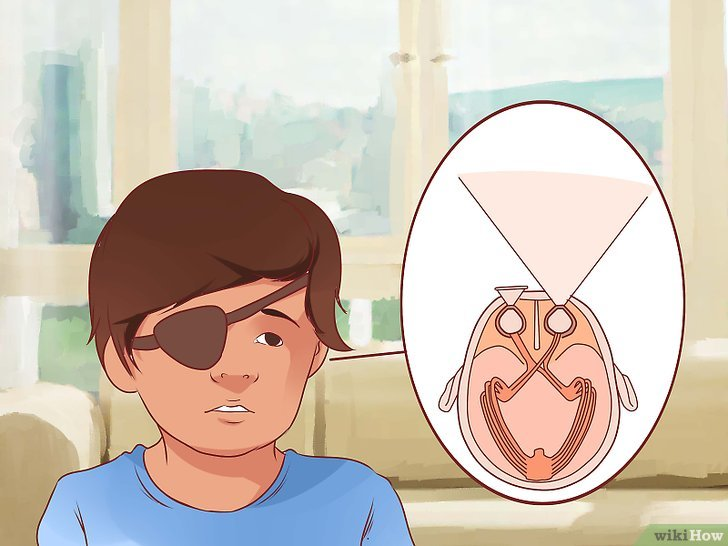
\includegraphics[width=60mm]{metoccl.jpg}
	 	\caption{Bendaggio occlusivo sull'occhio sano}
	 	\label{fig:metoccl}
	 \end{figure}
 
    \subsection{Atropina}
    Un' alternativa all'occlusione tramite un bendaggio vi è la penalizzazione farmacologica dell'occhio sano tramite una somministrazione di atropina.\\
    L'atropina è un tropan-alcaloide\footnote{famiglia di alcaloidi che contengono un anello tropanico nella loro struttura chimica.} impiegato per la produzione di un particolare collirio in grado di provocare la dilatazione della pupilla, effetto richiesto in occasione di interventi diagnostici e chirurgici sull'occhio, nonché nel trattamento di alcune malattie infiammatorie dell'occhio.\\
    Nel caso di ambliopia, la penalizzazione farmacologica mediante l'impiego di atropina impedisce l’accomodazione dell’occhio sano, promuovendo così l'utilizzo dell'occhio ambliope per oggetti vicini.\\
    Inizialmente questa terapia è stata utilizzata per ambliopia lieve poichè è stata giudicata insufficiente per il miglioramento di ambliopie più gravi. Recentemente però, attraverso studi scientifici, è stato dimostrato che la cura attraverso la dilatazione della pupilla porta notevoli progressi anche in casi di ambliopie importanti.
    \begin{figure}[h]
    	\centering   	
    	
\includegraphics[width=60mm]{atrop.jpg}
    	\caption{Somministrazione di atropina sull'occhio sano}
    	\label{fig:atrop}
    \end{figure}

    \subsection{Metodo I-BiT}
    University of Notthingham ha in corso un progetto per il trattamento dell'ambliopia indirizzato soprattutto per i pazienti più giovani: il progetto I-BiT (Interactive Binocular Treatment for Amblyopia).\\
    I-BiT consiste nello sviluppo di videogiochi interattivi basati sulla realtà virtuale, i quali devono avere i seguenti requisiti: 
    \begin{itemize}
    	\item Gli elementi secondari del gioco devono essere mostrati all'occhio sano;
    	\item Gli elementi principali del gioco devono essere mostrati esclusivamente all'occhio ambliope.
    \end{itemize}
	Ciò favorisce quindi di sfruttare di più le informazioni provenienti dall'occhio ambliope per avanzare nel videogioco.\\
	I-BiT è un metodo non ancora molto diffuso per via delle dimensioni ingombranti e degli elevati costi delle apparecchiature.
     \begin{figure}[h]
    	\centering   	
    	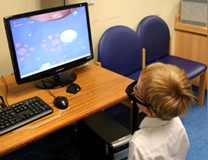
\includegraphics[width=60mm]{i-bit.jpg}
    	\caption{Un bambino sottoposto al metodo I-BiT}
    	\label{fig:ibit}
    \end{figure}
\newpage
\thispagestyle{empty}
    \chapter{3D4Amb}
    \section{Introduzione al progetto}
    3D4Amb è un progetto sviluppato dall'Università degli Studi di Bergamo che mira alla creazione di sistemi basati sulla tecnologia 3D active shutter\footnote{Tecnologia che consente di visualizzare immagini stereoscopiche 3D} per la diagnosi e il trattamento dell'ambliopia soprattutto nei bambini.\\
    La tecnologia 3D active shutter viene sfuttata per fornire una visione binoculare, ovvero mostrare immagini diverse all'occhio sano da quello ambliope. Ciò consente di effettuare diagnosi e trattamenti dell'ambliopia mediante giochi interattivi e attività di intrattenimento.\\
    Il progetto è coordinato dal prof. Angelo Gargantini con la collaborazione del Centro di ipovisione e riabilitazione visiva degli Ospedali Riuniti di Bergamo, del Policlinico di Milano e dell'Università degli Studi di Milano.
    \begin{figure}[h]
    	\centering   	
    	
\includegraphics[width=60mm]{logo3d4amb.png}
    	\caption{Logo ufficiale di 3D4Amb}
    	\label{fig:3d4amb}
    \end{figure}
    \section{Obiettivo del progetto}
    Come introdotto nel paragrafo precedente, 3D4Amb mira al svillupo di sistemi per la diagnosi e il trattamento dell'ambliopia. I principi fondamentali di tali sistemi, secondo le specifiche di 3D4Amb, devono essere:
    \begin{enumerate}
    	\item \textbf{\textit{Economicità}}: Il sistema deve poter essere utilizzato anche mediante l'uso di attrezzature e dispositivi poco costosi;
    	\item \textbf{\textit{Comodità}}: l'utilizzo del sistema può avvenire in qualsiasi ambiente e non per forza in centri specializzati o negli ospedali;
    	\item \textbf{\textit{Usabilità}}: Il sistema deve poter essere utilizzato facilmente da qualsiasi utente (soprattutto bambini);
    	\item \textbf{\textit{Divertimento}}: Il sistema deve intrattenere e divertire l'utente che lo sta utilizzando, alimentando così la sua propensione a collaborare. Il divertimento è un utile strumento che aiuta ad aumentare la probabilità di successo della diagnosi e trattamento dell'ambliopia. 
    \end{enumerate}
	Lo sviluppo di questi sistemi per il trattamento e la diagnosi dell'ambliopia consente di coniugare la cura e l'intrattenimento, processo difficilmente raggiungibile con i metodi tradizionali che spesso sono caratterizzati da uno scarso coinvolgimento da parte dei pazienti in età pediatrica e ciò comporta una diminuizione dei progressi durante la terapia.	
    \section{Tecniche}
    Il progetto 3D4Amb mira a sviluppare sistemi che consentono la visione binoculare, ovvero la visualizzazione di immagini differenti da parte dell'occhio sano e dell'occhio ambliope. In questo modo è possibile rendere visibile un'immagine con un maggior numero di dettagli all'occhio ambliope, mentre l'occhio sano visualizza un'immagine con meno particolari, obbligando così il cervello a raccogliere più informazioni dall'occhio ambliope (\figurename \ref{fig:visione}).
     \begin{figure}[h]
    	\centering   	
    	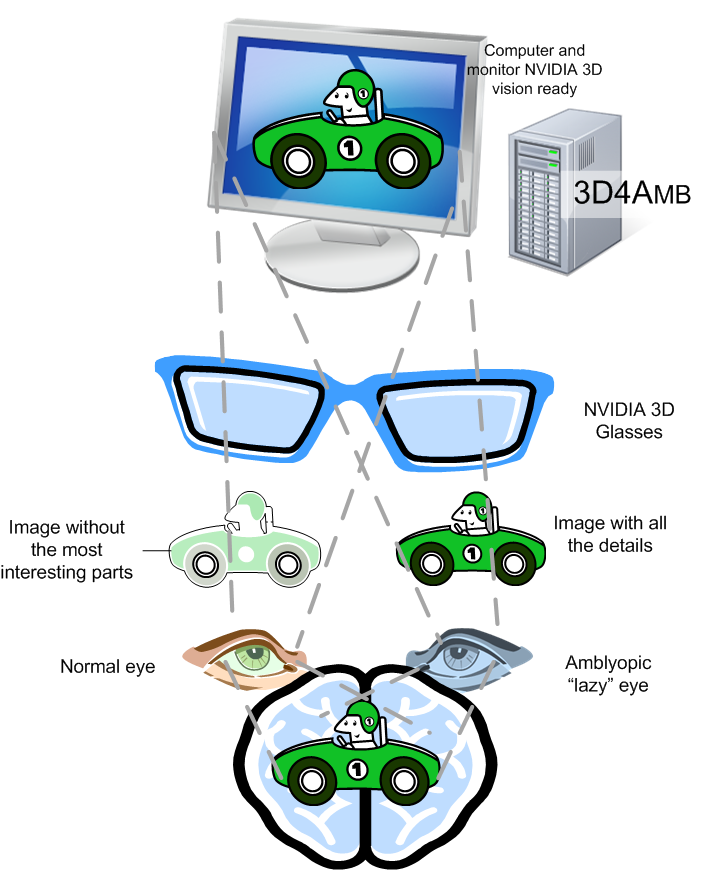
\includegraphics[width=7cm, height=9cm]{visione.png}
    	\caption{Utilizzo della tecnologia 3D in 3D4Amb}
    	\label{fig:visione}
    \end{figure}
    \subsection{Tecnica con anaglifi}
    L'anaglifo è un immagine stereoscopica che, se osservata con appositi occhiali (come quelli in \figurename \ref{fig:anagl}), fornisce un illusione di tridimensionalità.\\
    Per creare un immagine anaglifica vengono riprese due immagini parallele con due telecamere alla stessa distanza degli occhi umani (dai 6,5 cm a 7 cm). Una delle due immagini viene filtrata con il colore rosso (che è un colore sottrattivo) mentre l'altra viene filtrata con un filtro complementare (come il ciano, il blu e il verde che sono colori additivi). Infine si uniscono le due immagini e si stampa l'anaglifo, oppure è possibile proiettare le due immagini simultaneamente.\\ Visualizzare l'anaglifo a occhio nudo però non è agevole e non si percepisce l'illusione della tridimensionalità. Se però si visualizza l'immagine con appositi occhiali dove si ha una lente rossa e una lente filtrata con un colore additivo si percepisce una profondità dell'immagine che in realtà non esiste: l'occhio che vede attraverso il filtro rosso vedrà le parti di immagine rosse come parti "chiare", mentre l'occhio che vede attraverso il filtro ciano scarta le parti rosse e vede le parti dell'immagine ciano come parti "scure", così da fornire la tridimensionalità dell'immagine. 
    \begin{figure}[h]
    	\centering
    	 \subfloat{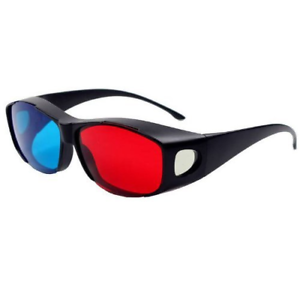
\includegraphics[width=.30\columnwidth]{anaglif.png}} \quad
    	\subfloat{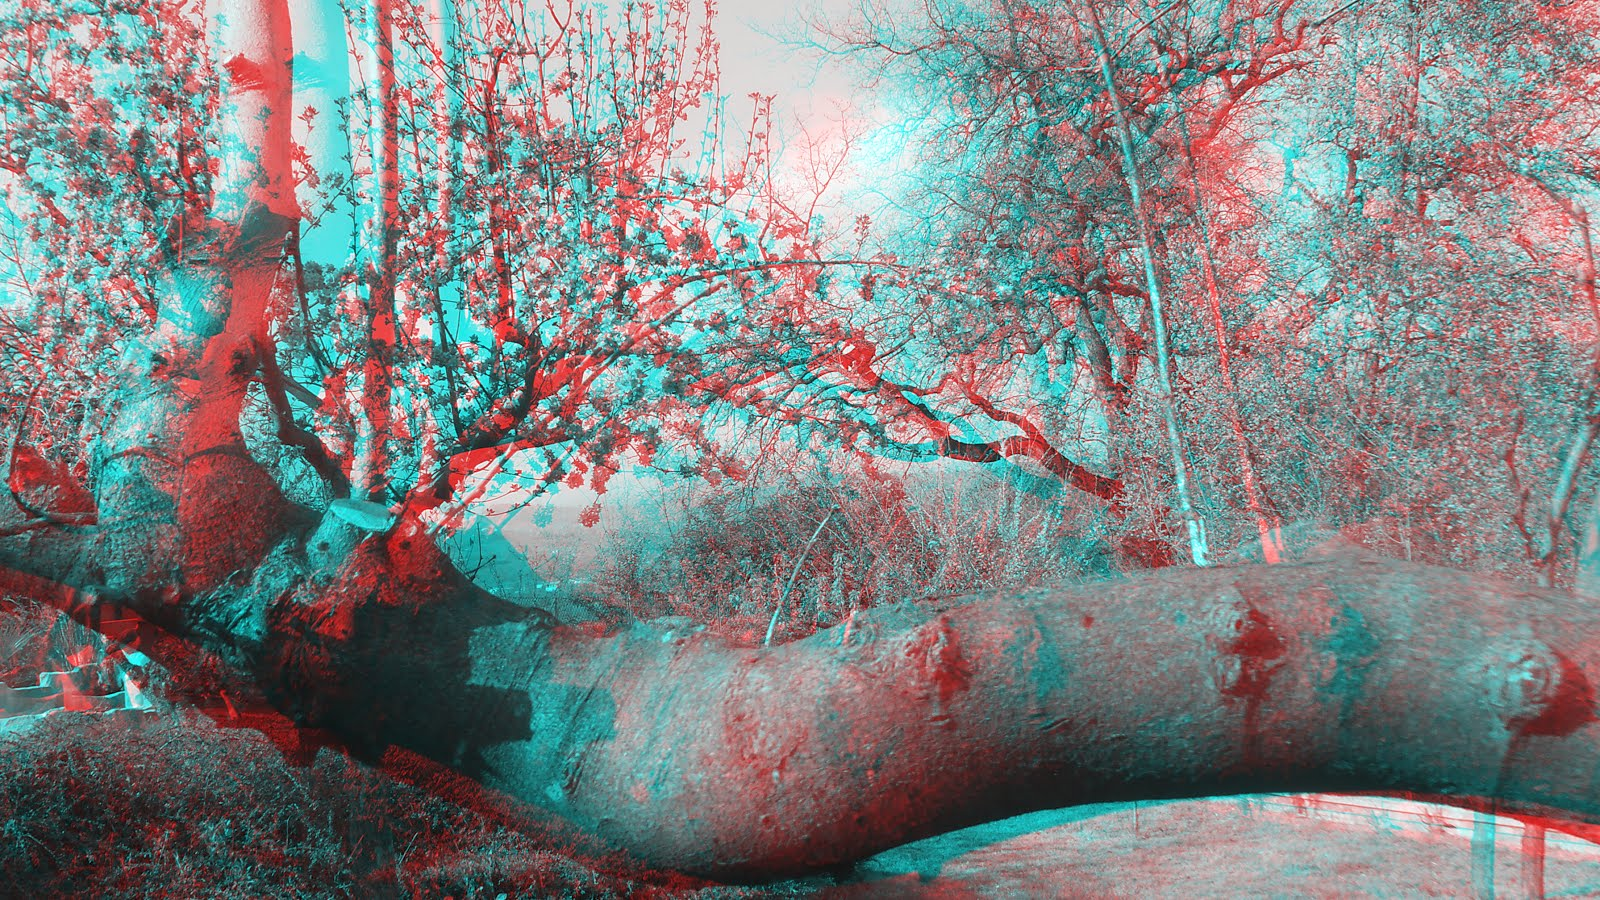
\includegraphics[width=.30\columnwidth]{ramanag.jpg}}
    	\caption{A sinistra occhiali per anaglifi. A destra immagine trasformata in anaglifo}
    	\label{fig:anagl}
    \end{figure}
\newpage
    \subsection{Tecnica Active Shutter}
    Una tecnica alternativa, ma simile, a quella anaglifica è l'utilizzo di occhiali 3D.\\
    Anche in questo caso occorre una ripresa di due immagini da due telecamere poste ad una distanza pari a quella tra due occhi. La visione delle due immagini deve essere simultanea ed ogni occhio deve poter vedere solo l'immagine ad esso destinata, in questo modo è possibile dare un'illusione di tridimensionalità. La visione simultanea delle due immagini è possibile grazie alla proiezione in rapida sequenza dei frame destinati alternativamente all'occhio destro e al sinistro e la distinzione delle immagini avviene attraverso un dispositivo ottico che permette l'otturazione in sincronia con i frame proiettati sullo schermo.\cite{wiki:3dglass} \\
     \begin{figure}[h]
    	\centering
    	\subfloat{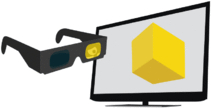
\includegraphics[width=.30\columnwidth]{frame-1.jpg}} \quad
    	\subfloat{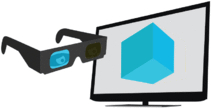
\includegraphics[width=.30\columnwidth]{frame-2.jpg}}
    	\caption{Principio di funzionamento di occhiali Active Shutter}
    	\label{fig:shutter}
    \end{figure}
	\subsection{Tecnica con visori VR}
	Un'altra possibile tecnica per la visione binoculare è quella mediante l'utilizzo di un visore VR. Essi sono dispositivi a forma di occhiali che permettono di percepire un'immagine proiettata su uno schermo come un immagine a realtà aumentata.\\
	Vi sono due tipologie di visori: quelli più sofisticati (come \textit{Oculus Rift} e \textit{Playstation VR}) che richiedono di essere collegati a potenti pc o console, oppure visori dove occorre semplicemente inserire uno smartphone nello scompartimento frontale (come \textit{Google Cardboard}).\\
	In questo caso creare una visione binoculare adatta a un trattamento dell'ambliopia è più semplice: bisogna duplicare una stessa immagine e penalizzare solo quella destinata all'occhio sano.
	\begin{figure}[h]
		\centering   	
		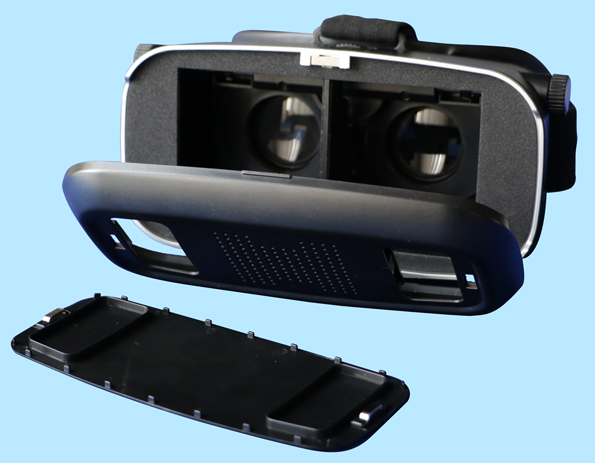
\includegraphics[width=30mm]{visorevr.jpg}
		\caption{Esempio di un visore VR con scompartimento frontale per smartphone}
		\label{fig:headsetvr}
	\end{figure}
	\chapter{Clash Ninja: Studi preliminari}
	\section{L'idea}
	Per un trattamento dell'ambliopia che coinvolge il paziente e che quindi permette di tenere alta la sua propensione a collaborare, 3D4Amb si occupa anche della realizzazione di videogiochi basati sulla tecnica di visione binoculare.\\
	Come si è visto in precedenza, la penalizzazione dell'immagine destinata all'occhio sano mediante l'utilizzo di un visore è il metodo più semplice: occorre sviluppare un videogioco con duplicamento dell'immagine e fornire meno dettagli a una delle due.\\
	Il videogioco sarà indirizzato principalmente a bambini perciò risulta decisivo creare un ambiente di gioco che catturi l'interesse e che sia in grado di far divertire, occorre dunque selezionare accuratamente la più adatta rappresentazione grafica di ogni elemento di gioco.\\
	Inoltre per incentivare un prolungato utilizzo del videogioco occorre l'introduzione di un sistema di gestione dei punteggi che spinge il giocatore a migliorare la propria prestazione di gioco. Al contrario, un gioco story driven\footnote{Giochi che seguono il filo logico di una storia conclusiva.} avrebbe previsto lo svolgimento di una storia all'interno del videogioco e una volta raggiunta la conclusione sarebbe impossibile per il giocatore continuare il videogioco e ciò significherebbe segnare la fine della terapia.\\
		\begin{figure}[h]
		\centering   	
		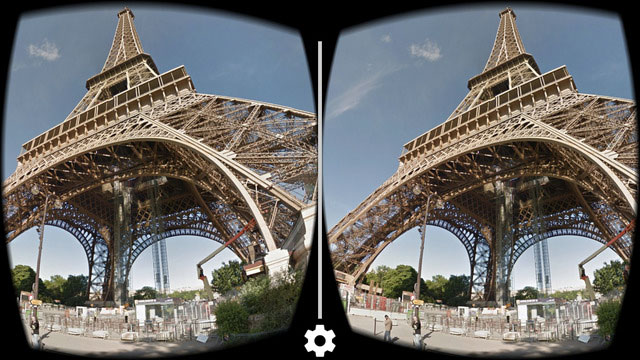
\includegraphics[width=50mm]{doubleimg.jpg}
		\caption{Duplicazione dell'immagine, tecnica utilizzata per il VR}
		\label{fig:doubleimg}
     	\end{figure}
     
	\section[Struttura]{Struttura di Clash Ninja}
	Clash Ninja è un gioco d'azione in 2D dove l'obiettivo è quello di sconfiggere il maggior numero di nemici. Lo si può definire un gioco \textit{survival}, ovvero dove bisogna resistere il più possibile agli attacchi dei nemici.\\
	Il protagonista del gioco è un ninja dotato di una spada che può saltare e attaccare. Il ninja ha 10 punti vita che si decrementano a ogni attacco del nemico andato a buon fine e si incrementano quando vengono raccolte delle pozioni sparse nella scena. Se si raggiunge la soglia minima di 0 punti vita il ninja viene sconfitto e la sessione di gioco si conclude.\\
	Il punteggio tiene conto dei nemici sconfitti: un nemico sconfitto corrisponde a 1 punto.\\
    Il gioco è suddiviso in tre scene con ambientazioni, dinamiche e nemici diversi:
    \begin{itemize}
    	\item Scena 1: ambientata in una pianura dove si aggirano degli arcieri scheletro che scaglieranno delle frecce contro il ninja. Le frecce, se colpiscono il ninja, tolgono 1 punto vita;
    	\item Scena 2: ambientata in un paesaggio vulcanico sorvegliato da guerrieri drago che alla vista del ninja scagliano delle palle di fuoco. Ogni palla di fuoco toglie 2 punti vita;
    	\item Scena 3: ambientata in un deserto dove risiedono stregoni che lanciano incantesimi. Se il ninja viene colpito perde 3 punti vita.
    \end{itemize}
		Il primo scenario è immediatamente disponibile, mentre si può accedere alla scena 2 una volta ottenuti, in almeno una sessione di gioco, 20 punti, corrispondenti alla sconfitta di 20 nemici. Il terzo ed ultimo scenario viene reso disponibile quando viene raggiunta la soglia dei 30 punti in una sessione di gioco.
		\begin{figure}[h]
		\centering   	
		
\includegraphics[width=60mm]{logoclashninja.png}
		\caption{Logo di Clash Ninja}
		\label{fig:logclash}
	\end{figure}	
	\section[Strumenti]{Strumenti utilizzati}
	Per realizzare un videogioco occorre un game engine, ovvero un nucleo software con grafica in tempo reale che fornisce strumenti per la modellizzazione delle scene di gioco e lo scripting. In questo caso la scelta del game engine da utilizzare è ricaduta su Unity.\\
	L'obiettivo di Clash Ninja, oltre a intrattenere i bambini come qualsiasi altro videogioco, è quello di procurare a un paziente affetto da ambliopia uno strumento di terapia coinvolgente. Per questo motivo è necessario implementare nel videogioco un meccanismo che permette la visione di un immagine meno dettagliata all'occhio sano per dare maggiore importanza alle informazioni acquisite dall'occhio ambliope. Tale meccanismo deve essere realizzato tramite una delle tecniche descritte nel capitolo precedente; in questo caso la scelta è ricaduta sullo sdoppiamento delle immagini, perciò lo strumento fondamentale per l'uso del videogioco è un visore VR.
	\subsection{Unity}
	Unity è un game engine sviluppato dalla Unity Technologies per la realizzazione di videogiochi 3D e 2D multipiattaforma. Infatti i videogiochi realizzati con Unity possono essere eseguiti su Microsoft Windows, Mac, Linux, IOS, Android, Xbox, Playstation e Nintendo; ciò lo rende tra i più famosi e utilizzati tanto da vantare una percentuale alta di impiego nel settore del videogame developing\footnote{Processo di produzione di un videogioco} mediante un motore grafico da terze parti (circa il 45\%).\\
	L'ambiente di sviluppo Unity è composto da:
	\begin{itemize}
		\item Motore grafico che permette di sviluppare la grafica in tempo reale;
		\item Motore fisico che permette di costruire la fisica del gioco;
		\item Live Game Preview, ovvero un'anteprima del gioco in tempo reale che viene utilizzata per testare il gioco in fase di sviluppo.
	\end{itemize}
	\begin{figure}[h]
	\centering
	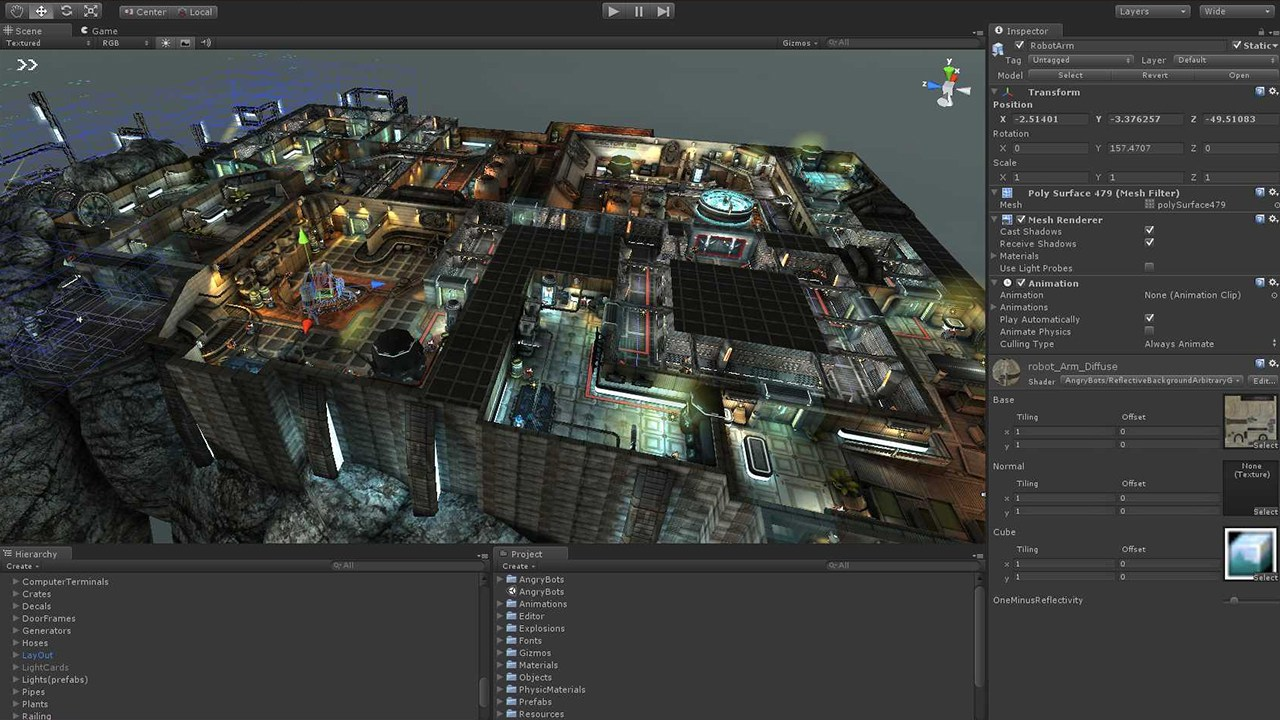
\includegraphics[width=100mm]{unity3D.jpg}
	\caption{Schermata principale di Unity}
	\label{fig:unity3d}
    \end{figure}
    Il game engine Unity permette lo sviluppo di un videogioco con un approccio ibrido tra il code-intensive, ovvero l'occorrenza di codice per gestire determinate operazioni, e il no-code per le azioni semplici (ad esempio il posizionamento degli elementi di gioco).\\
	Il linguaggio di programmazione di Unity è chiamato \textit{UnityScript} ed è sviluppato in due linguaggi: C\# e Javascript. Javascript è un linguaggio poco tipizzato e orientato agli oggetti, ma è comunque comodo per lo scripting del comportamento degli elementi di gioco. Mentre C\# è un linguaggio fortemente orientato agli oggetti e la sua struttura e la sua sintassi prendono spunto da linguaggi molto famosi come C++ e Java. Proprio per questo motivo, nel mondo di Unity, il linguaggio di programmazione più utilizzato per lo scripting è C\#.\\
	Gli elementi di gioco in Unity vengono realizzati grazie a oggetti con particolari proprietà denominati \textit{GameObject}. Le entità di gioco (come la telecamera, il giocatore, il nemico e la piattaforma su cui saltare) sono GameObject caratterizzati da un nome, dalla posizione nello spazio (che è possibile configurare inserendo le coordinate nel componente \textit{Transform}) e da componenti aggiuntivi. Le proprietà di un GameObject sono definite dai componenti, i quali possono essere dei script, collider, sorgenti di suoni ecc...\\
	\begin{figure}[h]
		\centering
		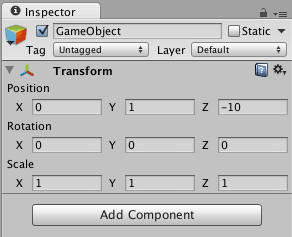
\includegraphics[width=70mm]{gameobject.png}
		\caption{Proprietà del GameObject}
		\label{fig:gameobject}
	\end{figure}
	\subsection{3D4Amb-ULib}
	Tra i progetti di 3D4Amb vi è lo sviluppo di una libreria che facilita la realizzazione di applicazioni videoludiche in Unity che possono fare da trattamento per l'ambliopia, il quale prende il nome di 3D4Amb-ULib.\\
	La libreria permette lo sdoppiamento automatico dei GameObject e permette la definizione della politica di gioco e della penalizzazione. Inoltre include un sistema di salvataggio dei punteggi delle sessioni di gioco di ogni giocatore e una schermata del menu principale personalizzabile con colori e testi adatti al proprio gioco che si sta sviluppando.	Per permettere ciò, 3D4Amb-ULib definisce dei GameObject adatti che devono essere importati nel proprio progetto Unity.\\
	Le politiche di gioco e della penalizzazione possono essere configurate dallo sviluppatore attraverso i GameObject \textit{PrefManager} e \textit{PenaltyManager}; con essi è possibile scegliere come gestire i livelli di difficoltà del gioco, che in questo caso specifico consiste nell' aumentare o diminuire l'intensità della penalizzazione dell'immagine vista dall'occhio sano.
	\subsection{Google Cardboard}
	Il videogioco utilizza la tecnica di penalizzazione mediante la duplicazione dell'immagine, perciò occorre l'utilizzo di un visore VR per giocare.\\
	Per testare Clash Ninja si è deciso di utilizzare \textit{Google Cardboard} poichè è un visore accessibile a tutti (il prezzo è circa di 7\euro).\\
	Google Cardboard è un visore low cost composto da cartone, pensato e realizzato da Google per incentivare la nascita di nuove start up attive nel settore della realtà virtuale.\\
	La sua caratteristica principale è la semplicità: per poterlo utilizzare occorre inserire lo smartphone nello scompartimento frontale e indossarlo. Grazie alle lenti interne che allargano l'immagine fino a coprire tutto il campo visivo, il giocatore percepisce la sensazione della realtà aumentata.\\
	Per giocare a Clash Ninja la scelta del visore da utilizzare non è comunque vincolata, ma è possibile utilizzarne uno qualsiasi.
	
	\begin{figure}[h]
		\centering
		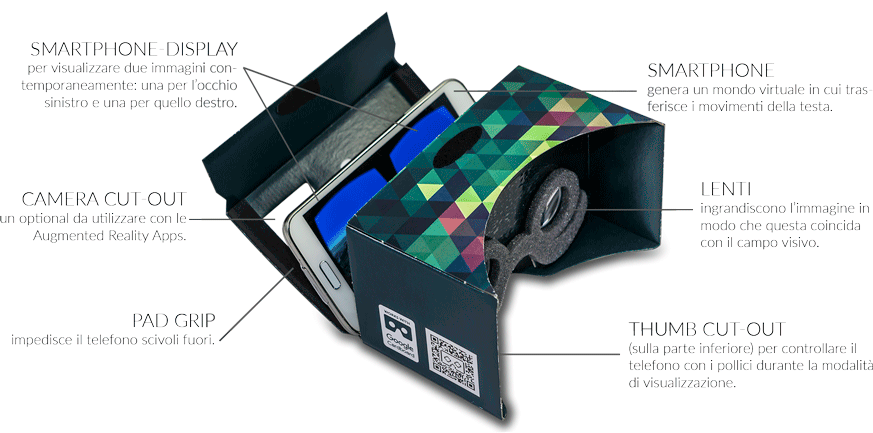
\includegraphics[width=120mm]{googlecardboard.png}
		\caption{Google Cardboard}
		\label{fig:cardboard}
	\end{figure}
	\subsection{Controller Bluetooth}
	Data la scelta di optare per il visore, Google Cardboard, che non vincola l'utente a utilizzare un visore con comandi esterni, occorre rendere il gioco comandabile da un controller che può interagire con lo smartphone con connessione Bluetooth.\\
	Anche in questo caso si può scegliere un qualsiasi controller Bluetooth con l'unica avvertenza di assicurarsi di acquistare un controller dotato di modalità di gioco.\\
	Il controller utilizzato per la fase di test di Clash Ninja è il \textit{Pyrus Bluetooth Controller}, il quale è dotato di un tasto analogico per il movimento del personaggio e 4 tasti che saranno utilizzati per il comando del salto, dell'attacco e della pausa del gioco. Pyrus Bluetooth Controller è un controller Bluetooth a basso costo (circa 8\euro) e quindi accessibile a tutti.\\
	\begin{figure}[h]
		\centering
		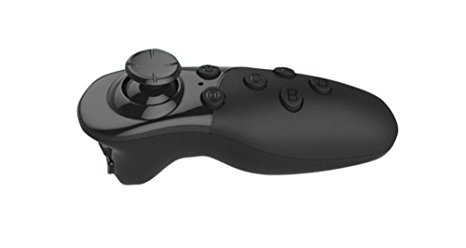
\includegraphics[width=50mm]{pyruscontroller.jpg}
		\caption{Pyrus Bluetooth Controller}
		\label{fig:pyruscontroller}
	\end{figure}
	Unity supporta in maniera nativa e molto intuitiva gli input provenienti da sorgenti diverse (come la tastiera, un joystick, tap su schermo, controller Bluetooth o USB) e li interpreta in maniera corretta. Ciò è possibile grazie a \textit{Input Manager}, dove è possibile definire il tipo di input e i comandi che può supportare il videogioco. Per dettagli sulla configurazione dei comandi in Input Manager che è stata adottata per lo sviluppo di Clash Ninja si rimanda al prossimo capitolo.
	\begin{figure}[h]
		\centering
		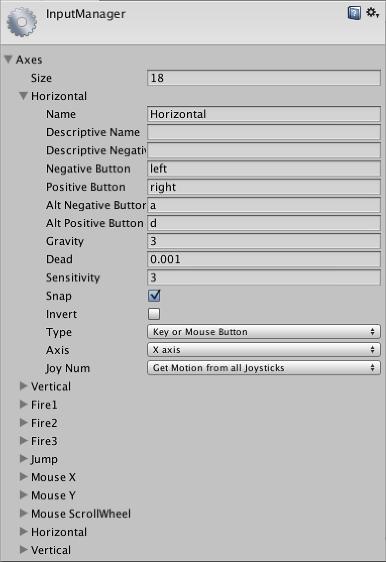
\includegraphics[width=40mm]{inputmanager.png}
		\caption{Input Manager di Unity}
		\label{fig:inputmanager}
	\end{figure}
\newpage
	\section{Set di gioco}
	In \figurename \ref*{fig:gameset} vi è un esempio di come è possibile utilizzare il sistema: l'utente affetto da ambliopia dovrà inserire lo smartphone nel visore e dovrà dotarsi di un controller Bluetooth. È consigliato però utilizzare un visore dotato di un elastico per sorreggerlo sulla testa così da impiegare entrambe le mani per il controller.
	\begin{figure}[h]
		\centering
		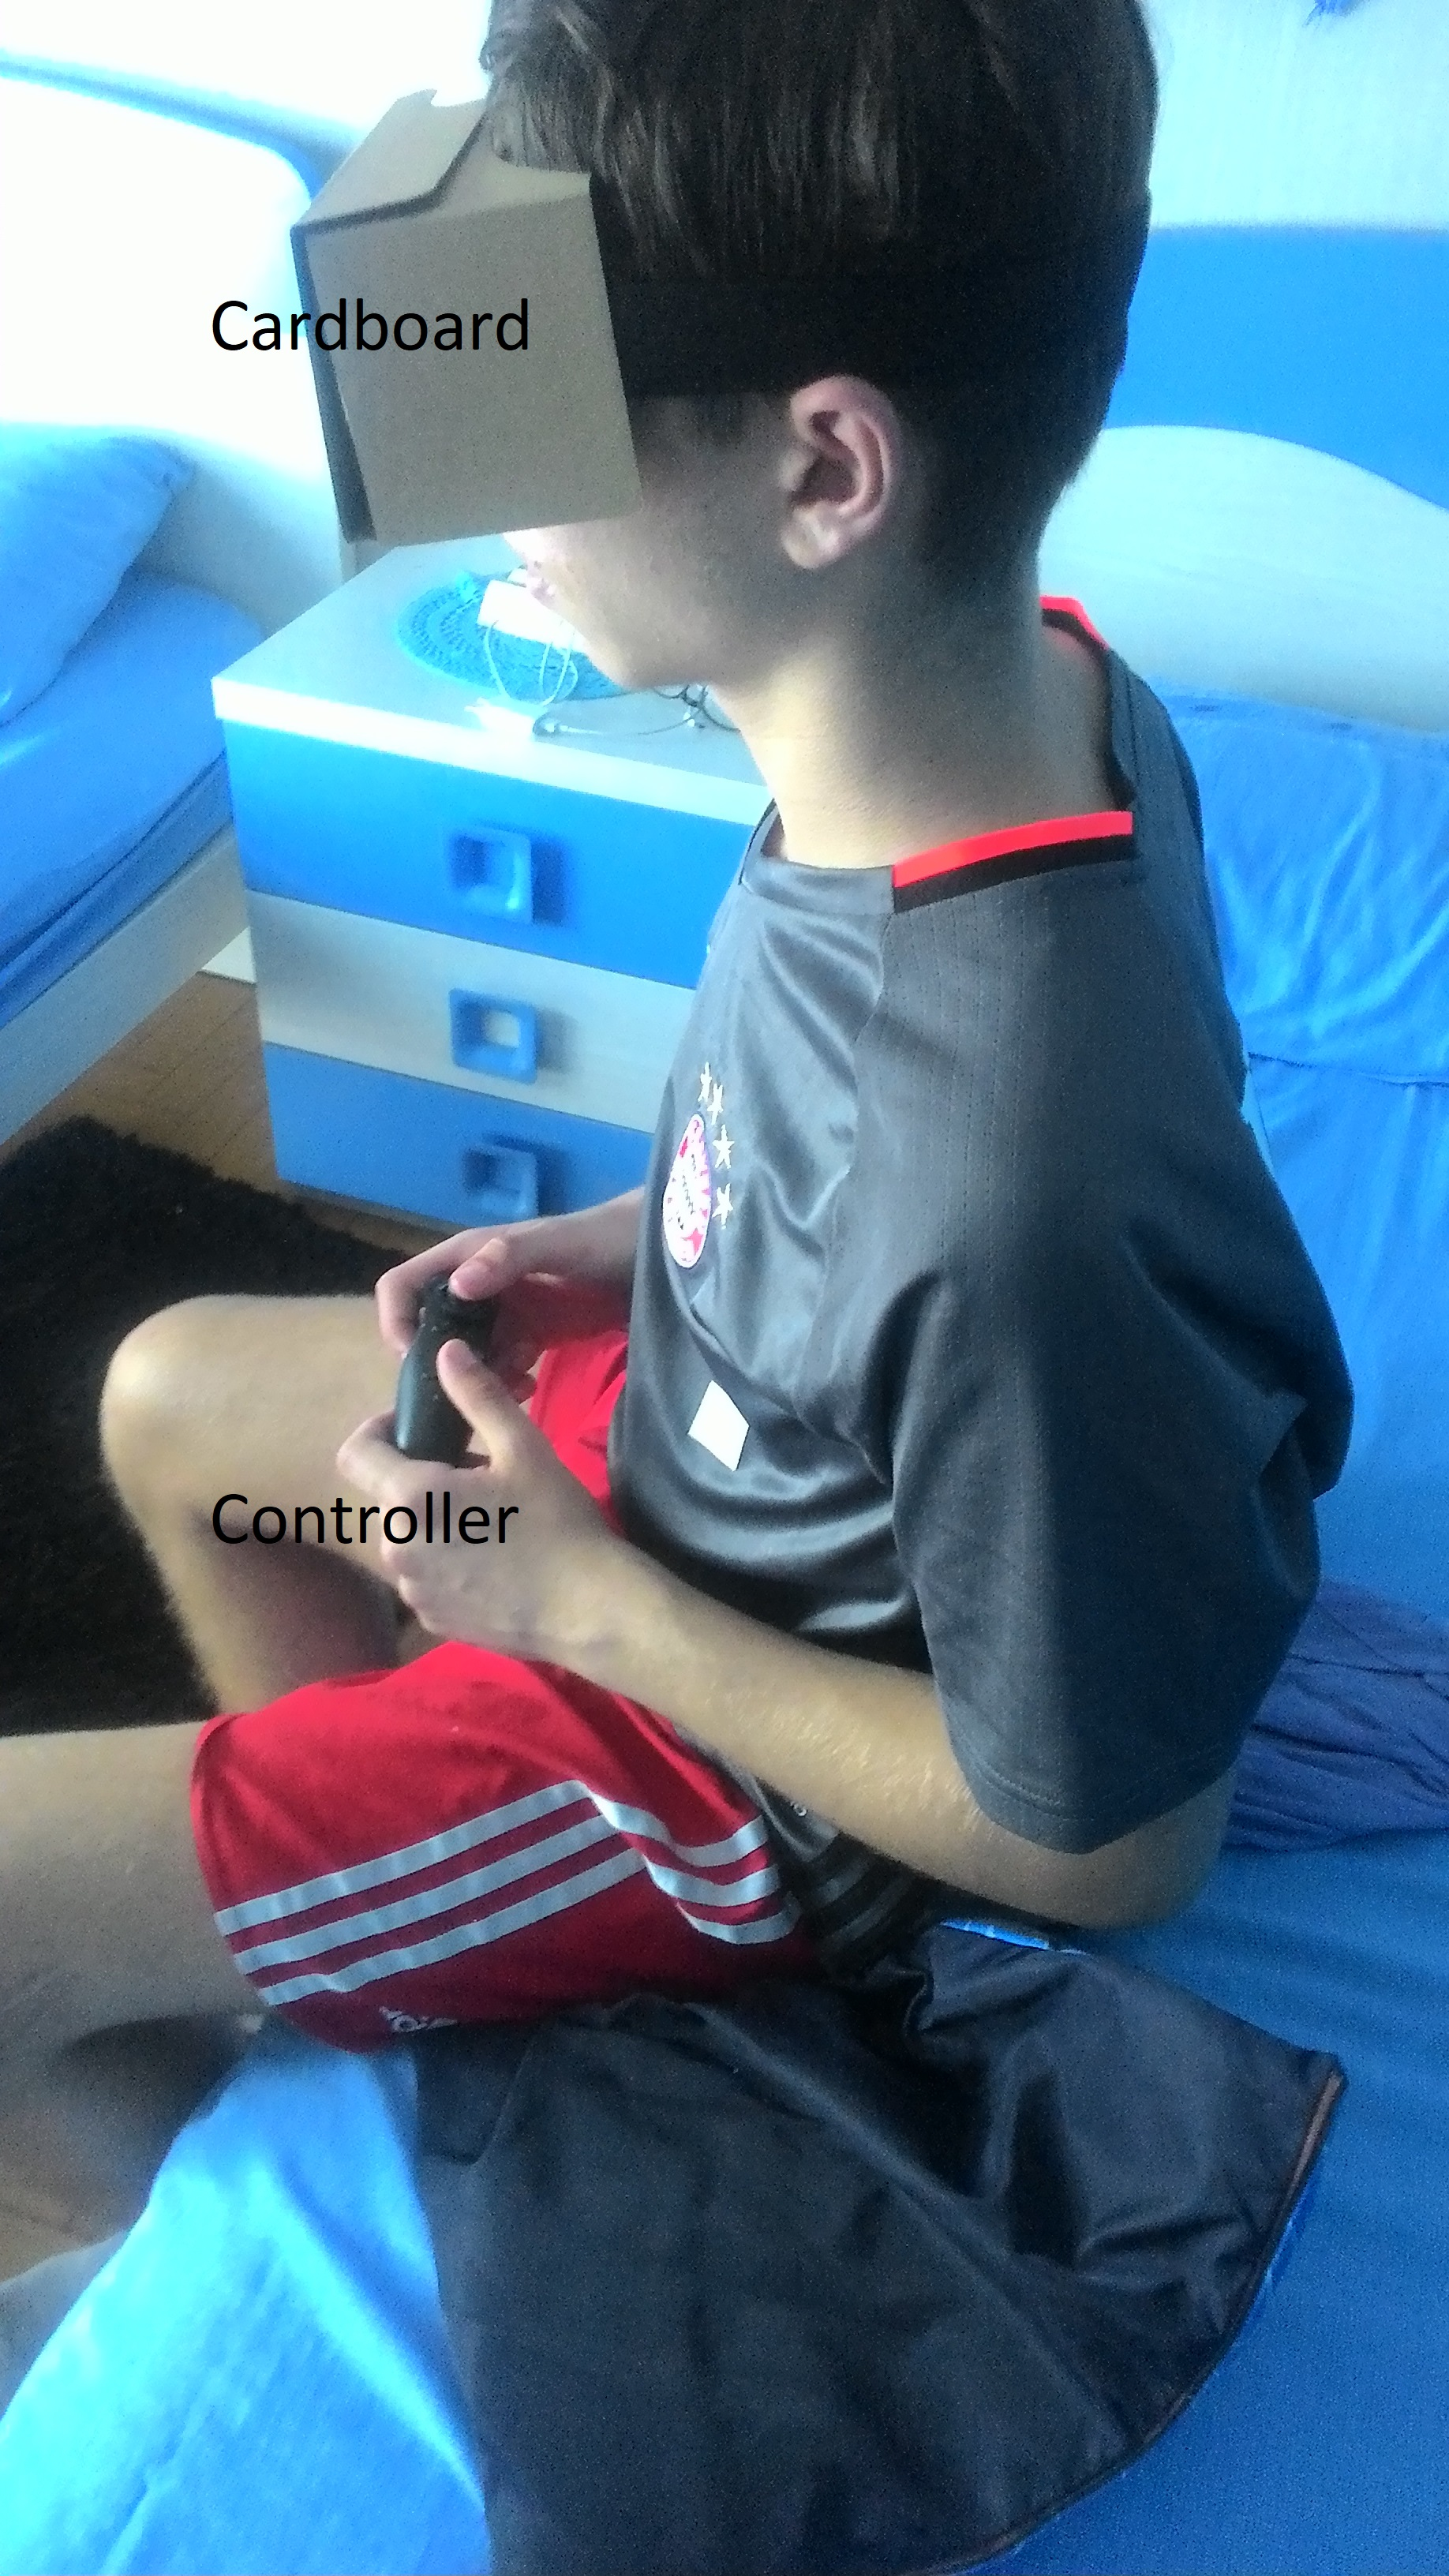
\includegraphics[width=40mm]{gameset.jpg}
		\caption{Set di gioco necessaria per Clash Ninja}
		\label{fig:gameset}
	\end{figure}
\newpage
\thispagestyle{empty}
	\chapter{Clash Ninja: Realizzazione}
	\section{Introduzione}
	Per lo sviluppo di Clash Ninja, come indicato nel precedente capitolo, è stato utilizzato il game engine Unity e il linguaggio scelto per lo scripting è C\#.\\
	La duplicazione dell'immagine, la maschera e la penalizzazione vengono implementate grazie alla libreria 3D4Amb-ULib che, importato nel progetto, permette anche di configurare la politica di penalizzazione e delle difficoltà del gioco.\\
	Si spiegheranno inoltre i punti critici della realizzazione del videogioco e le soluzioni adottate sui problemi riscontrati (ad es. il movimento del personaggio, l'intelligenza artificiale dei nemici e la gestione delle collisioni).\\
	
	\section[Sprite]{Sprite dei personaggi e ambienti}
	
	\subsection{Personaggio principale}
	\subsection{Nemici}
	\subsection{I mondi}
	\section{Collider}
	\section[Movimento]{Movimento del personaggio}
	\subsection{Gestione delle animazioni con mecanim}
	\subsection{Script del movimento}
	\section[AI del nemico]{Intelligenza artificiale del nemico}
	\subsection{Animazioni del nemico con mecanim}
	\subsection{Script per l'AI del nemico}
	\section{Spawning}
	\subsection{Generazione automatica dei nemici}
	\subsection{Generazione automatica delle pozioni}
	\section[3D4Amb-ULib]{Importazione di 3D4Amb-ULib}
    \bibliographystyle{plain}
    \bibliography{BibliografiaTesi}
\end{document}